\documentclass[a4paper, 10pt, twocolumn, twoside]{book}
\usepackage[dvipdfx, rgb]{xcolor}
  \definecolor{yellowtext}{HTML}{f9b00b}
  \definecolor{redtext}{HTML}{931004}
  \definecolor{whitetext}{gray}{0.5}
  
  \definecolor{normalpage}{gray}{0.95}
  \definecolor{storyblack}{gray}{0.1}
  \definecolor{boxred}{HTML}{721a16}
  \definecolor{headred}{HTML}{5e1519}

\usepackage{tikz}
\usetikzlibrary{fadings}
\usetikzlibrary{patterns}
\usetikzlibrary{external}
\usetikzlibrary{calc}
%\tikzexternalize[prefix=figures/]


\usepackage{geometry}
  \geometry{a4paper, 
  includeheadfoot,
  top=0cm, 
  headheight=23mm, 
  headsep=7mm, 
  footskip=23mm, 
  bottom=7mm,
  left=20mm, 
  right=15mm
  }  
  
\graphicspath{{./SR5_Fankit/}}
  
%  
  

\pagestyle{empty}
\begin{document}
\begin{tikzpicture}[remember picture, overlay, shift={(current page.center)}]

	\tikzstyle{reverseclip}=[insert path={(current page.north east) --
  (current page.south east) --
  (current page.south west) --
  (current page.north west) --
  (current page.north east)}
]

	\coordinate (TL) at (-87.5mm, 60mm);
 	\coordinate (BL) at (-87.5mm, -60mm);
 	\coordinate (BR) at (87.5mm, -60mm);
 	\coordinate (TR) at (87.5mm, 60mm);

	%\node at (0,0) {
\includegraphics[height=12cm, width=17.5cm]{image.png}};
	\begin{scope}	
	\clip ($(TL) + (1mm, 0mm)$) -- ($(TL) + (1mm, -5mm)$) -- ($(TL) + (6mm, 0mm)$) -- cycle [reverseclip];
	\clip ($(BR) + (-1mm, 0mm)$) -- ($(BR) + (-1mm, 5mm)$) -- ($(BR) + (-6mm, 0mm)$) -- cycle [reverseclip];
	\clip ($(TL) + (10mm, 0mm)$) -- ($(TL) + (1mm, -9mm)$) -- ($(BL) + (1mm, 3.53553mm)$) -- ++(-45:5mm) -- ($(BR) + (-10mm, 0mm)$) -- ($(BR) + (-1mm, 9mm)$) -- ($(TR) + (-1mm, -3.53553mm)$) -- ++(135:5mm) -- cycle [reverseclip];
	\fill[fill=boxred] ($(TL) + (-1mm, 0)$) -- ($(BL) + (-1mm, 0)$) -- ($(BR)+(1mm, 0)$) -- ($(TR)+(1mm,0)$) -- cycle;
	\begin{scope}
	\clip ($(TL) + (-2mm, 5mm)$) -- ++(0,-3cm) -- ++(-45:5mm) -- ++(0,-3.5cm)-- ++(-135:5mm) -- ($(BL)+(-2mm,0.53553mm)$) -- ++(-45:5mm) -- ($(BR) + (-33mm, -3mm)$) -- ($(BR) + (-28mm, -4mm)$) -- ($(BR) + (2mm, -4mm)$) -- ++(0,3.4cm) -- ++(135:5mm) -- ++(0,4cm) -- ++(45:5mm) -- ($(TR)+(2mm, -0.53553mm)$) -- ++(135:5mm) -- ++(-12.9cm, 0) -- ($(TL) + (37mm, 5mm)$) -- cycle;
	\node at (0,0) {
\includegraphics[width=\paperwidth, height=\paperheight]{Hintergruende/Skyline_Seattle_schwarz_1920x1080px.jpg}};
	\node[opacity=.2] at (0,1mm) {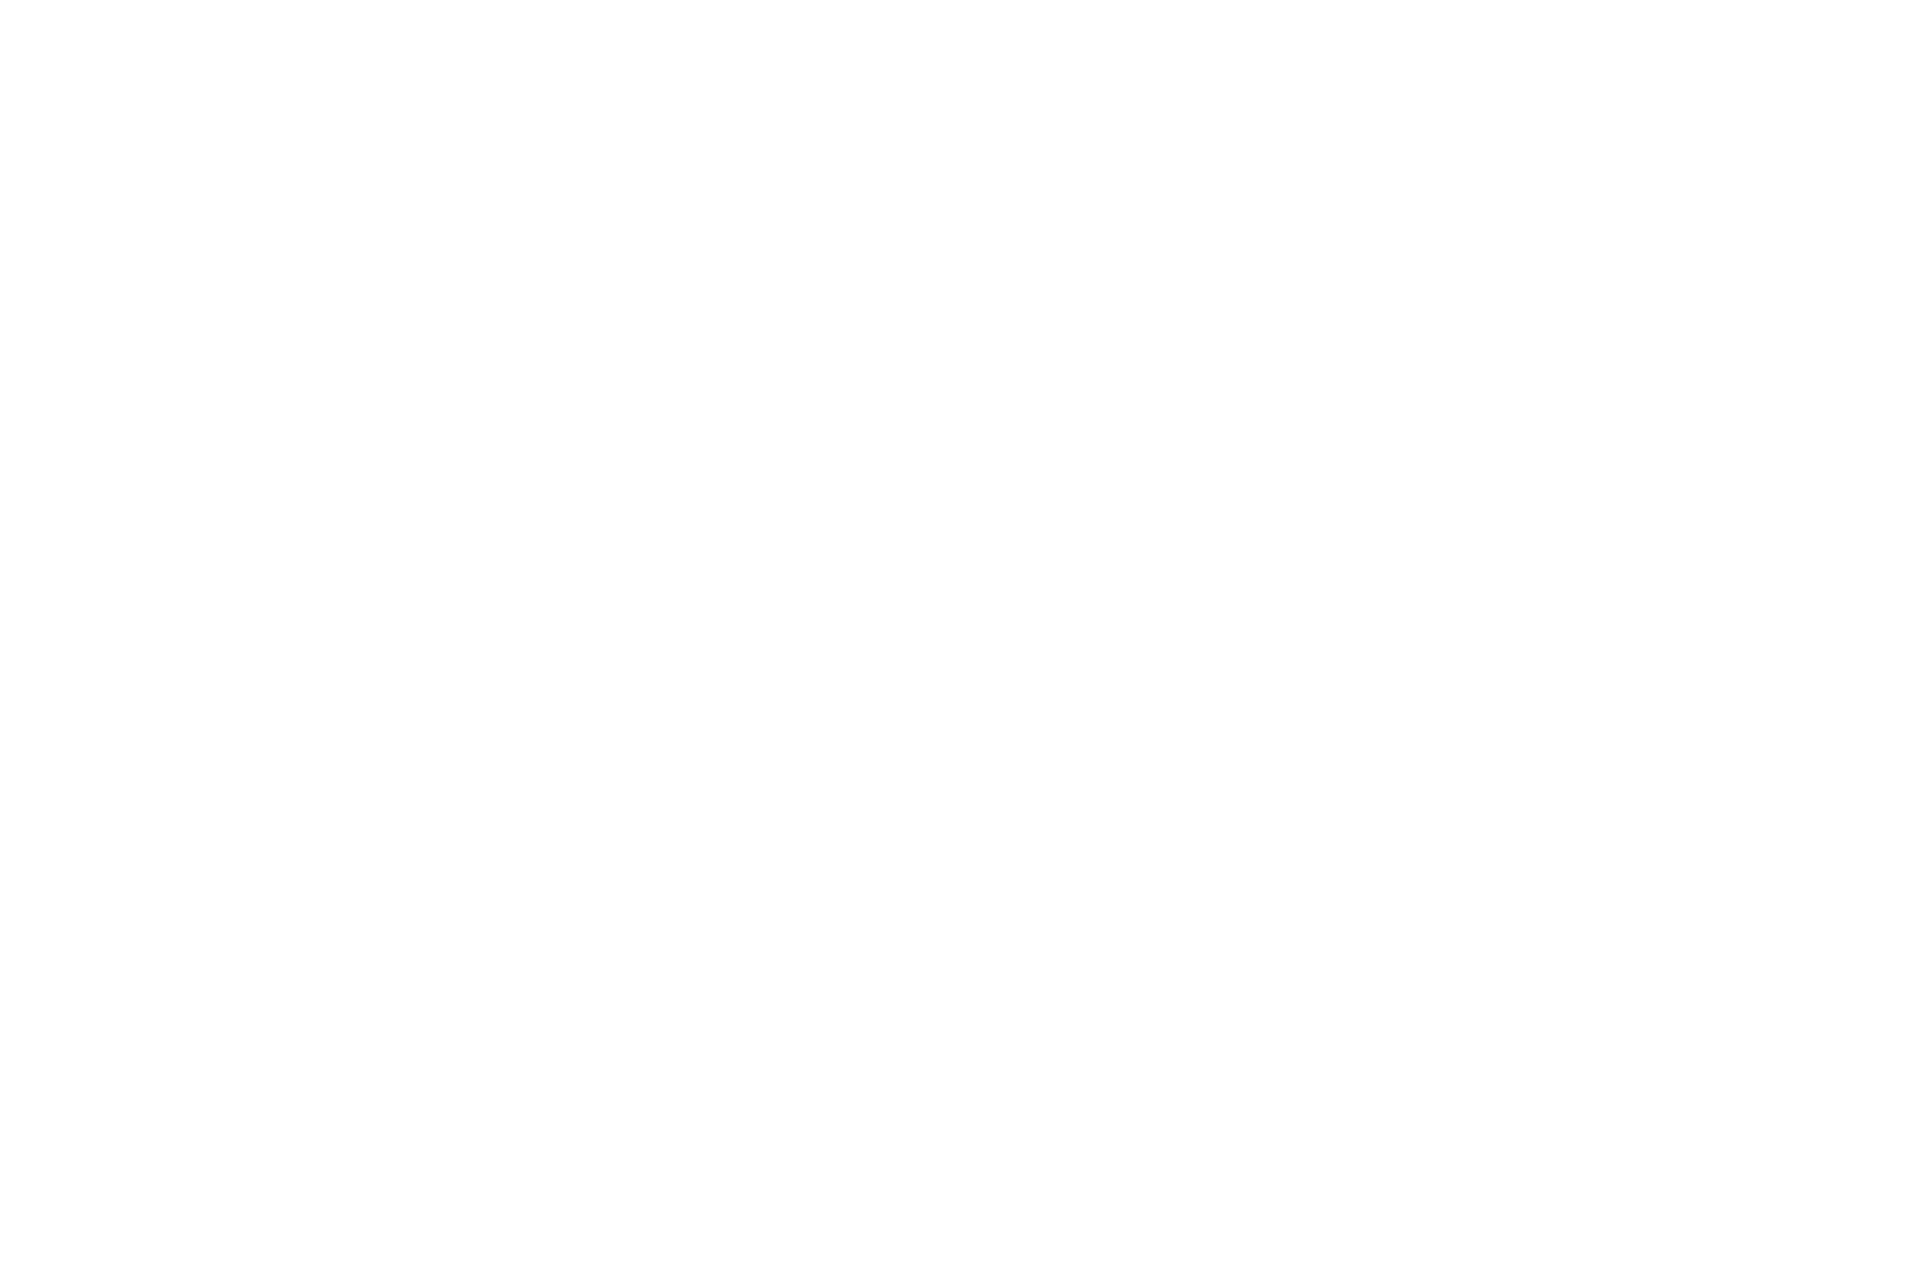
\includegraphics[width=20cm, height=14cm]{Hintergruende/Interface_1920x1280px.png}};
	\end{scope}
	\draw[draw=white, line width=.2mm] ($(TL) + (-2mm, 5mm)$) -- ++(0,-3cm) -- ++(-45:5mm) -- ++(0,-3.5cm)-- ++(-135:5mm) -- ($(BL)+(-2mm,0.53553mm)$) -- ++(-45:5mm) -- ($(BR) + (-33mm, -3mm)$) -- ($(BR) + (-28mm, -4mm)$) -- ($(BR) + (2mm, -4mm)$) -- ++(0,3.4cm) -- ++(135:5mm) -- ++(0,4cm) -- ++(45:5mm) -- ($(TR)+(2mm, -0.53553mm)$) -- ++(135:5mm) -- ++(-12.9cm, 0) -- ($(TL) + (37mm, 5mm)$) -- cycle;
	\end{scope}
	\draw[boxred, line width=.2mm] ($(TL) + (1mm, 0mm)$) -- ($(TL) + (1mm, -5mm)$) -- ($(TL) + (6mm, 0mm)$) -- cycle;
	\draw[boxred, line width=.2mm] ($(BR) + (-1mm, 0mm)$) -- ($(BR) + (-1mm, 5mm)$) -- ($(BR) + (-6mm, 0mm)$) -- cycle;
	\draw[boxred, line width=.2mm] ($(TL) + (10mm, 0mm)$) -- ($(TL) + (1mm, -9mm)$) -- ($(BL) + (1mm, 3.53553mm)$) -- ++(-45:5mm) -- ($(BR) + (-10mm, 0mm)$) -- ($(BR) + (-1mm, 9mm)$) -- ($(TR) + (-1mm, -3.53553mm)$) -- ++(135:5mm) -- cycle;
	\filldraw[draw=white, line width=.02mm, fill=boxred, opacity=.5] ($(TL) + (3mm,2.5mm)$) circle (1mm);
	\filldraw[draw=white, line width=.02mm, fill=boxred, opacity=.5] ($(TL) + (6mm,2.5mm)$) circle (1mm);
	\filldraw[draw=white, line width=.02mm, fill=boxred, opacity=.5] ($(TL) + (9mm,2.5mm)$) circle (1mm);
	
\end{tikzpicture}
\end{document}